\section{Spawning tasks}
\label{sec:spawn}

PFunc allows parallel execution of functions.  Let us explore this notion in a
bit more detail.  A normal function call is executed sequentially.
Furthermore, a sequence of function calls are also executed sequentially.
However, it is often the case that there are function calls that can be
executed at the same time without any harmful side effects.  In such cases, one
can make use of PFunc to execute functions in parallel with respect to each
other.  For example consider the problem of calculating the sum of an integer
array.

\begin{lstlisting}
int array_sum (int a[], int n) {
  int sum = 0;
  int i;
  for (i=0; i<n; ++i)  sum += a[i];

  return sum;
} 
\end{lstlisting}

Now, suppose that we are to sum up an array of 100 elements. We could then 
invoke \func{array_sum} as shown below:

\begin{lstlisting}
int main () {
  int a[100];
  return array_sum (a, 100);
}
\end{lstlisting}

Although this serves our purpose, we could speed up the calculation by 
splitting the array into two and using \func{array_sum} on each part:

\begin{lstlisting}
int main () {
  int a[100];
  return array_sum (a, 50) + array_sum (a+50, 50);
}
\end{lstlisting}

Once we have written the problem in this form, we can see that the two 
invocations of \func{array_sum} can actually be executed in parallel. It is
precisely such things that PFunc allows us to do.

\subsection{Creating work}
In the introductory section above, we saw what PFunc allows us to do.
However, the term \textbf{function} is broad, and as such, PFunc can only accept
functions expressed in a particular form. In this section, we exposit on the
functions that PFunc accepts. In brief, PFunc accepts work in two forms: as
function pointers (C and \Cpp{}), and function objects (\Cpp{} only).  In this
section, we explain the functions and function pointers that are accepted by
PFunc.

\begin{figure}
\centering
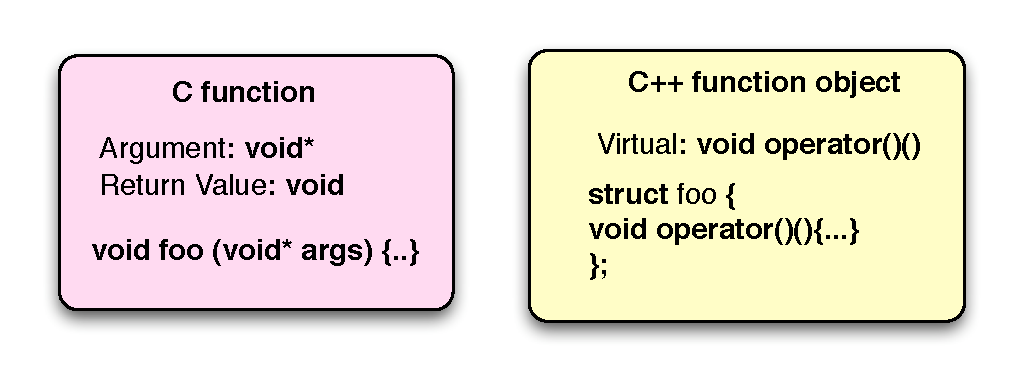
\includegraphics[width=0.6\textwidth]{figs/functors}
\caption{Prototypes of work accepted by PFunc.}
\label{fig:functors}
\end{figure}

\subsubsection{C-style function pointers}
PFunc accepts function pointers of the type \code{void (*)(void*)}. The
example below demonstrates how one such function looks like.

\begin{lstlisting}
void parallel_foo (void* arg) {
  char* string = (char*) arg;
  printf ("PFunc task printing: %s\n", string);
  return;
}
\end{lstlisting}

Note that the function only accepts a single argument of type \code{void*}.
Because of the constraints of a statically typed language, PFunc cannot accept
arbitrary function objects as tasks.  However, PFunc provides two function
calls - \func{pfunc_pack} and \func{pfunc_unpack} to facilitate currying
arguments to parallel functions (see Section~\ref{sec:pack}).

\subsubsection{\Cpp{} function objects}
PFunc also accepts \Cpp{} function objects (overloaded \func{operator()}) as
work. Figure~\ref{fig:functors} depicts the prototype of function objects.
However, using function objects as work requires some attention. As function
objects name concrete types, users must decide if they have more than one
\code{type} of function object that needs to be parallelized. If so, then 
all the function objects must derive from a common base class, which can then
be used as the type of the \code{Function object} feature during library 
instance generation (see Section~\ref{sec:generate}). In the following 
sections, we explain how to generated library instance descriptions for both 
cases.

\begin{list}{\labelitemi}{\leftmargin=1em}
\item \textbf{Single function object:} In this case, for optimal performance, 
it is beneficial to explicitly name the function object that is going to be 
used at library instance description generation time. For example, consider 
the code sample given below:

\begin{lstlisting}
/* Forward declaration */
struct parallel_foo;

/* Library instance description */
typedef pfunc::generator<cilkS, /* scheduling policy */
                         pfunc::use_default, /* compare */
                         parallel_foo> my_pfunc; /*function object*/

struct parallel_foo {
  ...
  void operator()() { ... };
};
\end{lstlisting}

In this case, \code{parallel_foo} is the only function object that can be 
parallelized by the library instance \code{my_pfunc}. As the function object 
is explicitly named, PFunc avoids making virtual function calls when spawning 
tasks. Using one function object to parallelize suffices for many applications
(eg., Fibonacci in Section~\ref{sec:fibonacci}).

\item \textbf{Multiple function objects:} In this case, users are required to
name a common type during library instance description generation and have all
their function objects derive from this type.  To facilitate this case, PFunc
provides a built-in base type that users can derive from. The following example
demonstrates the use of the common base type:

\begin{lstlisting}
/* Library instance description */
typedef pfunc::generator<cilkS, /* scheduling policy */
                         pfunc::use_default, /* compare */
                         pfunc::use_default> my_pfunc; /*function object*/

/* First function object */
struct parallel_foo : public my_pfunc::functor {
  void operator()() { ... };
};

/* Second function object */
struct parallel_bar : public my_pfunc::functor {
  void operator()() { ... };
};
\end{lstlisting}

In the example above, \code{pfunc::use\_default} is used as the value for the
\code{Function object} feature. As a result, PFunc uses a virtual base class
that stipulates \func{operator()}. The type of this class can be accessed from
the generate library instance description using the nested type
\code{::functor}. Now, invocations of \func{operator()} on both
\code{parallel\_foo} and \code{parallel\_bar} can be parallelized.

\end{list}

\subsection{Spawning tasks}
Once we have initialized the library and created work (functions and function
objects), we can parallelize execution of these work packets using PFunc. In 
addition to the work packets, each task is comprised of three additional 
details. These are:

\begin{list}{\labelitemi}{\leftmargin=1em}
\item \code{Attribute:} controls the execution of the task (see
Section~\ref{sec:attribute}).  PFunc provides suitable default value to this
parameter.
\item \code{Group:} enables SPMD-style task groups (see
Section~\ref{sec:group}).  PFunc provides suitable default value to this
parameter.
\item \code{Task handle:} a receipt for the spawned task. This handle can be 
used to query the status of the spawned task.
\end{list}

In \Cpp{}, these types can be accessed as nested types of the generated library
instance description. In C, these types are pre-generated. 

\subsubsection{Spawning tasks in C}
\label{subsubsec:spawn_c}
In this section, we will introduce parallelization of a simple function using 
PFunc by means of an example. Consider the code sample give below.

\begin{lstlisting}
void parallel_foo (void* arg) {
  char* string = (char*) arg;
  printf ("PFunc task number: %s\n", string);
  return;
}

int main () {
  pfunc_cilk_task_t tasks[10];
  unsigned int num_queues = 4;
  const unsigned int num_threads_per_queue[] = {1,1,1,1};
  pfunc_cilk_taskmgr_t cilk_tmanager;
  int i;

  /* Initialize a global instance of the library */
  pfunc_cilk_taskmgr_init (&cilk_tmanager, num_queues, num_threads_per_queue, NULL);

  /* Spawn the tasks */
  for (i=0; i<10; ++i) {
    pfunc_cilk_task_init (&(tasks[i]));
    pfunc_cilk_spawn_c (cilk_tmanager, tasks[i], NULL, NULL, parallel_foo, ltoa(i));
  }

  /* Wait for the tasks and clear the task handle */
  for (i=0; i<10; ++i) {
    pfunc_cilk_wait (cilk_tmanager, tasks[i]);
    pfunc_cilk_task_clear (&(tasks[i]));
  }

  /* Clear the library */
  pfunc_cilk_taskmgr_clear (&cilk_tmanager);

  return 0;
}
\end{lstlisting}

In the above example, we have parallelized execution of \func{parallel_foo}
using PFunc. First, we initialize the Cilk-style library instance using the
function call \func{pfunc_cilk_taskmgr_init}. In this example, we use task
queues, 1 thread per queue and allow default values for thread affinities.
Second, we spawn 10 instances of \func{parallel_foo} using the function
\func{pfunc_cilk_spawn_c}. In this example, we choose to use the default value
(NULL) for both \code{attribute} and \code{group}. Notice that the task handle
has to be initialized (using \func{pfunc_cilk_task_init}) prior to its use in
\func{pfunc_cilk_spawn_c}. This is required as the C types are mere pointers to
their \Cpp{} counterparts. Third, we wait for the spawned tasks to finish using
\func{pfunc_cilk_wait} before clearing the task handles. Finally, we clear the
initialized library using \func{pfunc_cilk_taskmgr_clear}. This deallocates all
resources (threads and internal queues) that are in use by PFunc. Note that we 
could have use the global runtime facility provided by PFunc in this example
by setting up \code{cilk_tmanager} using \func{pfunc_cilk_init}.

\subsubsection{Spawning tasks in \Cpp{}}
\label{subsubsec:spawn_cxx}
In this section, we will parallelize the execution of a function object that is
equivalent to the function parallelized in the previous section. The code is 
given below:

\begin{lstlisting}
struct parallel_foo {
  void initialize (const int& _id) { id = _id; }
  void operator()() {
    std::cout << "PFunc task number:" << id << std::endl;
  }
  private:
  int id;
};

/* Library instance description */
typedef pfunc::generator<cilkS, /* scheduling policy */
                         pfunc::use_default, /* compare */
                         parallel_foo> my_pfunc; /*function object*/

int main () {
  my_pfunc::task tasks[10];
  parallel_foo work[10];
  unsigned int num_queues = 4;
  const unsigned int num_threads_per_queue[] = {1,1,1,1};

  /* Initialize an instance of the library */
  my_pfunc::taskmgr cilk_tmanager (num_queues, num_threads_per_queue);

  /* Make this instance the global runtime */
  pfunc::init (cilk_taskmgr);

  /* Spawn the tasks */
  for (int i=0; i<10; ++i) {
    work[i].initialize (i);
    pfunc::spawn (tasks[i], work[i]);
  }

  /* Wait for the tasks and clear the task handle */
  for (int i=0; i<10; ++i) pfunc::wait (tasks[i]);

  /* Clear the global runtime */
  pfunc::clear ();

  return 0;
}
\end{lstlisting}

This example has many changes from its C counterpart. First, notice that we do
not have to initialize objects such as \code{task}, \code{attribute} or
\code{group} as they are initialized on construction. Second, default values
for unused parameters such as \code{affinity} (for \func{pfunc::init}),
\code{attribute} and \code{group} (for \func{pfunc::spawn}) are filled in and
consequently, there is no need to explicitly pass their values. Finally,
notice that we use the global version of the functions \func{spawn} and
\func{wait} because we set up \code{cilk_tmanager} as our global runtime.

\subsubsection{Waiting on tasks}

\begin{figure}
\begin{center}
\begin{tabular}{|c|c|l|}
\hline
\Cpp{} & C & Brief \\
\hline
\func{pfunc::wait} & \func{pfunc_cilk_wait} & \\
                   & \func{pfunc_lifo_wait} & Wait till completion of the listed task. \\
                   & \func{pfunc_fifo_wait} & \\
                   & \func{pfunc_prio_wait} & \\
\hline
\func{pfunc::wait_all} & \func{pfunc_cilk_wait_all} & \\
                       & \func{pfunc_lifo_wait_all} & Wait till completion of all the listed tasks. \\
                       & \func{pfunc_fifo_wait_all} & \\
                       & \func{pfunc_prio_wait_all} & \\
\hline
\func{pfunc::wait_any} & \func{pfunc_cilk_wait_any} & \\
                       & \func{pfunc_lifo_wait_any} & Wait till completion of any one of the listed tasks. \\
                       & \func{pfunc_fifo_wait_any} & \\
                       & \func{pfunc_prio_wait_any} & \\
\hline
\func{pfunc::test} & \func{pfunc_cilk_test} & \\
                   & \func{pfunc_lifo_test} & Test for completion (non-blocking) of the listed task. \\
                   & \func{pfunc_fifo_test} & \\
                   & \func{pfunc_prio_test} & \\
\hline
\func{pfunc::test_all} & \func{pfunc_cilk_test_all} & \\
                       & \func{pfunc_lifo_test_all} & Test for completion of all the listed tasks. \\
                       & \func{pfunc_fifo_test_all} & \\
                       & \func{pfunc_prio_test_all} & \\
\hline
\end{tabular}
\end{center}
\caption{Different types of wait in PFunc.}
\label{fig:wait}
\end{figure}
In the examples seen till now, we used \func{pfunc::wait} (or
\func{pfunc_<schedpolicy>_wait}) to wait on spawned tasks. However, there are
multiple functions which allow users to check the status of spawned tasks.
These are summarized in Figure~\ref{fig:wait}. Using these new functions, the 
waiting portion of the code sample in 
Section~\ref{subsubsec:spawn_c} can be rewritten as follows:

\begin{lstlisting}
pfunc_cilk_wait_all (cilk_tmanager, tasks, 10);
\end{lstlisting}

Similarly, the waiting portion of the code sample in 
Section~\ref{subsubsec:spawn_cxx} can be rewritten as follows:

\begin{lstlisting}
pfunc::wait_all (tasks, 10);
\end{lstlisting}
